%====================================================================
\section{Annexe : premier essai d'AlphaFold3 sur l'ubiquitine}
\label{sec:ubiquitine}
%====================================================================

\paragraph{Protéine choisie.} Avant la prédiction de la calmoduline (section~\ref{sec:af3}), un premier essai a servi à valider la manipulation sur AlphaFold Server :
\begin{itemize}
  \item \textbf{Nom} : ubiquitine ; \textbf{organisme} : \emph{Homo sapiens} ;
  \item \textbf{Identifiant et base de données} : entrée PDB \textbf{1UBQ}, chaîne~A (RCSB PDB~\cite{berman2000}), structure obtenue par diffraction des rayons~X à 1,8~Å~\cite{vijaykumar1987} ; la même séquence correspond aux résidus 1 à 76 de l'entrée UniProtKB \textbf{P0CG47} (gène \emph{UBB})~\cite{uniprot_P0CG47} ;
  \item \textbf{Longueur} : \textbf{76 résidus} ; \textbf{séquence utilisée} :\\
  {\scriptsize\ttfamily MQIFVKTLTGKTITLEVEPSDTIENVKAKIQDKEGIPPDQQRLIFAGKQLEDGRTLSDYNIQKESTLHLVLRLRGG}
\end{itemize}
Cette protéine est plus courte que la plage recommandée (100 à 400 résidus). C'est volontaire : il s'agissait seulement de tester la chaîne de travail, avec un résultat rapide, sur une protéine dont la structure est très bien connue. Le calcul se faisant sur les serveurs de Google, le temps de calcul n'était pas une contrainte. Les résultats sont conservés dans \texttt{results/fold\_2026\_10\_27\_12\_32/} (la tâche a gardé le nom proposé par défaut) et la capture dans \texttt{figures/af3\_ubiquitine.png}.

\begin{figure}[H]
  \centering
  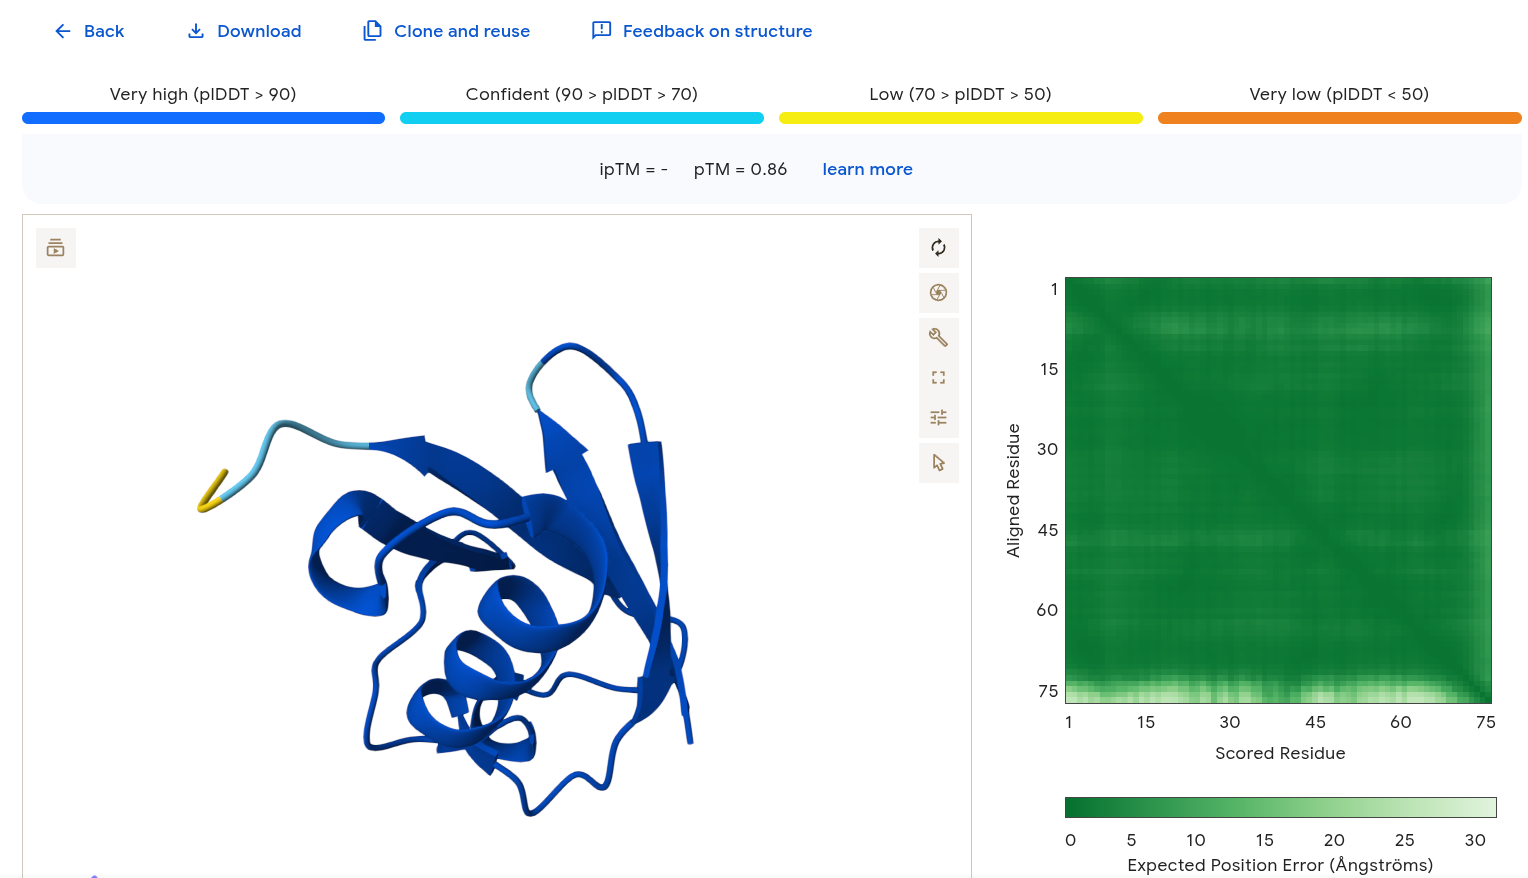
\includegraphics[width=0.8\textwidth]{../figures/af3_ubiquitine.png}
  \caption{Premier essai d'AlphaFold3 : l'ubiquitine (pTM = 0,86).}
  \label{fig:af3_ubiquitine}
\end{figure}

\paragraph{Résultat.} La structure montre le repliement \og $\beta$-grasp \fg{} caractéristique de l'ubiquitine : un feuillet $\beta$ enroulé autour d'une hélice $\alpha$ (figure~\ref{fig:af3_ubiquitine}). La confiance est très élevée : pTM de \textbf{0,86}, pLDDT moyen de \textbf{91,9}, 70 résidus sur 76 au-dessus de 90. Seule la queue C-terminale est moins sûre : son pLDDT décroît de 93 (Leu71) à 53 (Gly76), et la PAE qui la relie au reste de la protéine atteint 13,5~Å en moyenne, contre 1,7~Å dans le cœur. C'est cohérent avec la biologie : cette queue flexible se termine par la glycine~76, qui se lie de façon covalente aux protéines cibles lors de l'ubiquitination. L'ipTM n'est pas défini (\og ipTM = - \fg{}), puisqu'il n'y a qu'une seule chaîne.

Comme pour la calmoduline, le serveur a utilisé 4 gabarits contenant l'ubiquitine (6NJD, 3WXE, 5VIX et 5OE7). L'excellente prédiction était donc attendue : ce test montre que la chaîne de travail fonctionne, mais il ne mesure pas la capacité d'AlphaFold3 à prédire une structure inconnue.

